\section{Results}\label{sec:results}
\subsection{Surface Density Projections}\label{ssec:projections}
Before dissecting the simulated galaxies in detail, we first take a look at the surface density projections of the gas and stars in the central region, situated on the central galaxy in the bimodal simulation. This is shown in Figure~\ref{fig:projections}. In each grouping of four, the bottom and top rows show the face-on and edge-on views, respectively. The left and right columns show the gas (blue) and stellar (orange) surface density, respectively. Each panel is oriented with respect to the stellar angular momentum of the final snapshot ($t=8\,\Gyr$). The angular momentum is computed using all star particles within the half-mass radius.

We can see that the galaxy grows in size after the merger. Additionally, the galaxy's orientation continues to change even within the last $3\,\Gyr$. The final galaxy is oriented $\sim126\degree$ with respect to the initial orientation of the central galaxy's gas halo. The dynamical and kinematic consequences of such a gas-rich merger is beyond the scope of our current work.

\begin{figure*}
  \centering

    \gridline{\fig{all_L30/all_L30_frame60.pdf}{0.3\textwidth}{}
              \fig{all_L30/all_L30_frame70.pdf}{0.3\textwidth}{}
              \fig{all_L30/all_L30_frame80.pdf}{0.3\textwidth}{}
              }
    \gridline{\fig{all_L30/all_L30_frame90.pdf}{0.3\textwidth}{}
              \fig{all_L30/all_L30_frame100.pdf}{0.3\textwidth}{}
              \fig{all_L30/all_L30_frame110.pdf}{0.3\textwidth}{}
              }
    \gridline{\fig{all_L30/all_L30_frame120.pdf}{0.3\textwidth}{}
              \fig{all_L30/all_L30_frame200.pdf}{0.3\textwidth}{}
              \fig{all_L30/all_L30_frame320.pdf}{0.3\textwidth}{}
              }
  % \includegraphics[width=\textwidth]{surfdens.pdf}
  \caption{Frames from a movie showing a surface density projection of the bimodal simulation over time. In each frame, the left/right (blue/orange) column shows the gas/star surface density. The upper/lower panels show the edge-on and face-on view. Every panel is oriented with respect to the final ($t=8\,\Gyr$) snapshot. The side-length of each panel is $30\,\kpc$, and the image is a projection through a box with the same side-length. The colormap for the gas ranges from $1$ to $10^2\,\Msun/\pc^2$, while for the stars ranges from $1$ to $10^4\,\Msun/\pc^2$. (A full movie, also for the unimodal and isolated simulations, is here \red{TBD}.)}
  \label{fig:projections}
\end{figure*}

\subsection{Abundance Distribution}\label{ssec:abundplane}
In Figure~\ref{fig:fig1}, briefly discussed in Section~\ref{sec:intro}, we show the abundance distribution of the Milky Way as well as two of our idealized merger simulations in the upper panels. A number of our idealized simulations exhibit either a bimodal or unimodal abundance distribution, and so we have selected two representative examples. The simulation labeled bimodal had orbital parameters of $R_0=142\,\kpc$, $V_0=116\,\kms$, and $\eta=0.4$. The unimodal simulation is identical, except that $R_0=129\,\kpc$. The bimodal and unimodal labels are of the outcome of the simulation, and do not reflect any particular choice made in their setup.

There are, of course, differences between the bimodal simulation and the Milky Way. First, the scaling in \MgFe{} is different -- in the simulation, the low-$\alpha$ sequence lies at $\sim0.2$, while in the Milky Way it is at about $\MgFe\sim0$. Second, in the Milky Way the high-$\alpha$ sequence neatly joins the low-$\alpha$ sequence at $\FeH\sim0$, while in the simulation the two actually diverge more at higher \FeH{}. Finally, at high \FeH{} the distribution bends upwards while in the simulation it bends downwards.

In the lower panels of Figure~\ref{fig:fig1}, we show the distributions of \MgFe{} at different fixed \FeH{}. The (blue, orange, red, green) lines show the \MgFe{} distribution at a \FeH{} of ($-0.5$, $-0.25$, $0$, $0.25$), in bins of width $0.05\,\dex$. The distributions of \MgFe{} are offset (but not rescaled) so that they do not overlap. Here, the bimodality seen in the Milky Way is quite striking at lower metallicities. The peaks are well-separated, by $\sim0.2\,\dex$. In the bimodal simulation, the distribution is still clearly bimodal, but the peaks are less well-separated, by $\sim0.1\,\dex$. In the unimodal simulation, there is a hint of some structure at $\FeH \gtrsim 0.25$, but there is not a strong multimodal structure.

\subsection{Build up of the Abundance Plane}\label{ssec:abundplane_build}
Next, we examine the build up of the abundance plane. First, in Figure~\ref{fig:before_after}, we show the abundance plane at various points along the merger. We have divided the history of the merger into ``before'' ($t < 1.5\,\Gyr$), ``during'' ($1.5\,\Gyr < t < 2.5\,\Gyr$), and ``after'' ($t > 2.5\,\Gyr$). These times have been chosen somewhat by the orbital history and somewhat by visually inspecting the simulation, and so these deliniations are, to an extent, arbitrary. Nonetheless, it is clear that the high-$\alpha$ sequence forms before and during the merger (middle panels), and that the low-$\alpha$ sequence forms after the merger (right panel). We show a dashed line given by $-0.1\times\FeH + 0.31$, which is a crude way of separating the high- and low-$\alpha$ sequence.

It is informative to examine the star formation history (SFH) split into the high- and low-$\alpha$ sequences at a fixed \FeH{}, shown in Figure~\ref{fig:before_after_sfh}. The high- and low-$\alpha$ sequences (blue and orange) are defined as the star particles lying above and below the dashed line in Figure~\ref{fig:before_after}, respectively. We show this only in a narrow bin of width $0.1\,\dex$ at $\FeH\sim0$. We chose this value of \FeH{} because here the valley of the bimodality is deepest (see Figure~\ref{fig:fig1}). One can see a very clear separation in time between the high- and low-$\alpha$ sequences, with the high-$\alpha$ sequence forming before the low-$\alpha$ sequence.\footnote{There is a small amount of low-$\alpha$ formation at the very end of the high-$\alpha$ sequence, but this can be understood as simply an inadequacy in our simple way of separating the two sequences. Alternatively, one could assert that the separation in time is the real delineation between the two sequences, and that the boundary in the abundance plane has only mild contamination.} Furthermore, there is a brief period of $\sim300\,\Myr$ between the two sequences where no stars have formed.

It can also be shown that the exact timing of this quiescent period is metallicity-dependent. We show the same SFH in Figure~\ref{fig:before_after_sfh_by_iron}, but at varying bins in \FeH{} of $-0.5$, $-0.25$, and $0$ (blue, orange, and red, respectively). For clarity, we do not separate the SFHs by the high- and low-$\alpha$ sequences, but have verified that the same demarcation arises as in Figure~\ref{fig:before_after_sfh}. Here, we can see that at $\FeH=-0.5$ the quiescent period begins $\sim250\,\Myr$ earlier than at $\FeH=0$.

\subsection{\alphaFe{} Behavior Associated with Quiescence}
We now examine more closely the natural suspicion that the quiescent phase in Figure~\ref{fig:before_after_sfh} is responsible for the bimodal structure in Figure~\ref{fig:before_after}. In Figure~\ref{fig:SFR_alpha}, we show the SFR (blue lines) of each of the bimodal and unimodal galaxies (left and right panels, respectively) as well as the median \MgFe{} of the gas (orange lines) in a bin centered on $\FeH{}=-0.1$ with width $0.05\,\dex$. The SFR is shown for the entire galaxy ($r<15\,\kpc$) while the median \MgFe{} is shown for $2\,\kpc<r<5\,\kpc$.\footnote{The solar neighborhood-like selection of stars (discussed in Section~\ref{ssec:solarneigh}) mostly selects stars at $2\,\kpc<r<5\,\kpc$. We choose to plot the median \MgFe{} of the gas at these radii, since it is roughly that gas which is forming stars that ends up in our sample. On the other hand, we choose to show the SFR for the entire galaxy, as the enrichment from that star formation affects the entire galaxy at this epoch.}

The merger appears to induce a starburst, where the SFR rises from $\sim3.5\,\Msunyr$ at $\sim1\Gyr$ to a peak of $\sim12\,\Msunyr$ at $\sim2\,\Gyr$. This starburst is then followed by a quiescent period, with a minimum SFR of $\sim1\,\Msunyr$ and a duration of $\sim500\,\Myr$. The dip in SFR is not as pronounced as it was when we plotted the SFH at a particular iron (Figure~\ref{fig:before_after_sfh}). This quiescent period is associated with a drop in \MgFe{} from $\sim0.35$ to $\sim0.2\,\dex$ in only $\sim250\,\Myr$. Once the SFR recovers $\sim500\,\Myr$ later, \MgFe{} again rises, but only to $\sim0.28\,\dex$.

This behavior is absent in the unimodal simulation (right panel) -- while there is a starburst, it does not display a period of suppressed star formation, and there is no associated drop in \MgFe{}. It does still have a period of enhanced star formation, but this is actually coincident with an enhancement in \MgFe{}. This sequence of events is further emphasized in Figure~\ref{fig:alpha_vs_tform}, which shows a transparent scatter plot of \MgFe{} as a function of formation time. In the bimodal simulation, there is a clear gap in \MgFe{} during the period of quiescence followed by the brief formation of $\alpha$-deficient stars. In the unimodal simulation, on the other hand, there is no gap and instead a brief formation of $\alpha$-enhanced stars.

\subsection{Cause of Quiescence}\label{ssec:cause_qui}
Why there is a quiescent period in the bimodal simulation but not the unimodal simulation probably has to do with some transient, stochastic property of the gas in and around the galaxy. In some states, the AGN is better able to quench the galaxy than in others. Verifying this further is beyond the scope of this work, but we show some evidence of the association in Appendix~\ref{app:cause_qui}.

This outcome suggests that a merger alone is not sufficient in order to generate a bimodality. Rather, the merger must induce a quenching phase. Whether this occurs depends both on the properties of the merger but also on the state of the central galaxy itself and whether it can launch AGN-driven winds that result in significant gas removal. Our work would argue for some stochasticity in whether a particular merger leads to such quenching.

\begin{figure*}
  \centering
  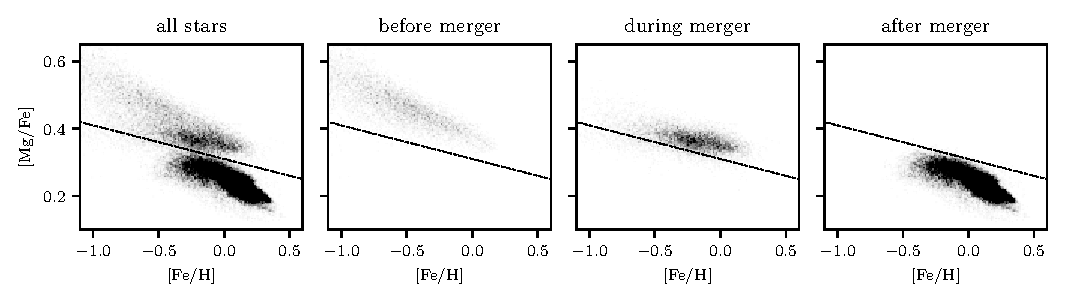
\includegraphics[width=\textwidth]{before_after.pdf}
  \caption{\textbf{The high-$\alpha$ sequence forms before the merger, the low-$\alpha$ sequence forms after the merger.} This plot shows the sequence of events leading to the build-up of the low- and high-$\alpha$ sequences for our fiducial bimodal simulation. We have separated the high- and low-$\alpha$ sequences by a dashed line at $-0.1\FeH + 0.31$, which was chosen by eye to lie in the trough. The left panel shows all star particles in our solar neighborhood cut. The middle left panel shows the star particles that form before the merger ($\tform < 1.5\,\Gyr$), which form a weak sequence of star particles at the lowest \FeH and highest \MgFe. The middle right panel shows the star particles that form during the starburst ($1.5\,\Gyr < \tform < 2.5\,\Gyr$). These star particles form the portion of the high-$\alpha$ sequence closest to the trough, and the density of star particless is higher than those that form before. The right panel shows the star particles which form after the merger ($\tform > 2.5\,\Gyr$). These star particles form almost entirely below the trough.}
  \label{fig:before_after}
\end{figure*}

\begin{figure}
  \centering
  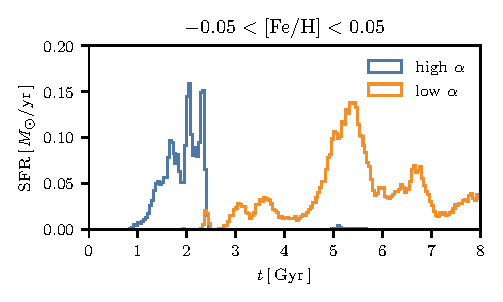
\includegraphics[width=\columnwidth]{before_after_sfh.pdf}
  \caption{\textbf{At fixed metallicity, the low- and high-$\alpha$ sequence are cleanly separated in time by an intervening quiescent period.} Here we show the star formation history of the high- and low-$\alpha$ sequences. The blue (low-$\alpha$) and orange (high-$\alpha$) histograms correspond to the dashed line cut made in the \MgFe{}-\FeH{} plane in Figure~\ref{fig:before_after}, at a fixed metallicity of $\FeH=0$ with width $0.05\,\dex$. One can see that there is a nearly perfect separation in time between the formation of the high-$\alpha$ and low-$\alpha$ sequences by a quiescent period lasting $\sim300\,\Myr$. There is a small amount of contamination at the end of the high-$\alpha$ sequence which can be attributed to the inadequacy of the linear cut model of the two sequences.}
  \label{fig:before_after_sfh}
\end{figure}

\begin{figure}
  \centering
  \includegraphics[width=\columnwidth]{before_after_sfh_by_iron.pdf}
  \caption{\textbf{The timing of the quiescent period which divides the high- and low-$\alpha$ sequences is metallicity dependent.} The star formation history of stars at various fixed metallicities ($\FeH=0$, $-0.25$, and $-0.5\,\textrm{dex}$) in bins of width $0.05\,\dex$. As in Figure~\ref{fig:before_after_sfh}, there is a quiescent period period which separates the formation of the low- and high-$\alpha$ sequence. However, the timing of the quiescent period is metallicity-dependent. It occurs earlier at lower metallicities, by $\sim250\,\Myr$ for the metallicities shown in this plot.}
  \label{fig:before_after_sfh_by_iron}
\end{figure}

\begin{figure*}
  \centering
  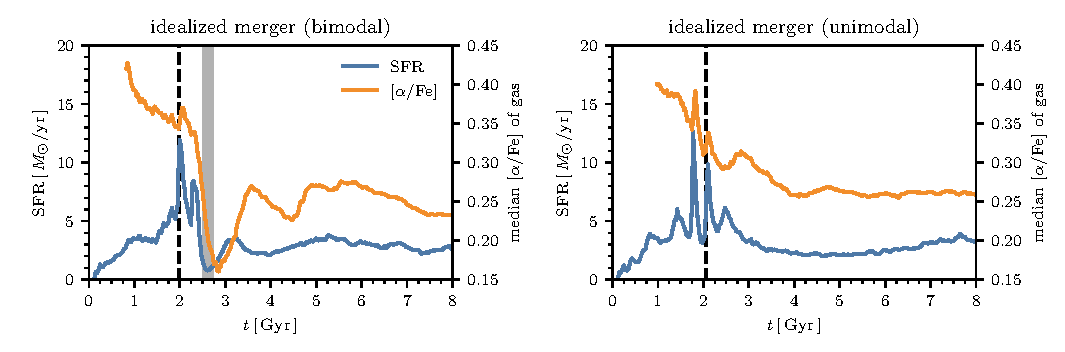
\includegraphics[width=\textwidth]{SFR_alpha.pdf}
  \caption{\textbf{A global suppression of star formation is associcated with a decrease in \MgFe{}, which is seen in the bimodal simulation but not in the unimodal simulation.} Here, we show both the SFR of the central galaxy ($r<15\,\kpc$) and the median \MgFe{} for gas at $2\,\kpc<r<5\,\kpc$ at a fixed \FeH{} bin centered on $0$ with width $0.05\,\dex$. The left panel shows the bimodal simulation while the right panel shows the unimodal simulation. A vertical dashed line at $2\,\Gyr$ in each plot indicates the approximate time of the merger, but before complete coalescence. In the left panel, a shaded region from $2.5\,\Gyr$ to $2.75\,\Gyr$ indicates the approximate period of quiescence shown in Figure~\ref{fig:before_after_sfh}. This suppression of star formation is associated with a sudden drop in the median \MgFe{} of the gas. Neither the suppression of star formation nor the drop in \MgFe{} are seen in the unimodal simulation.}
  \label{fig:SFR_alpha}
\end{figure*}

\begin{figure}
  \centering
  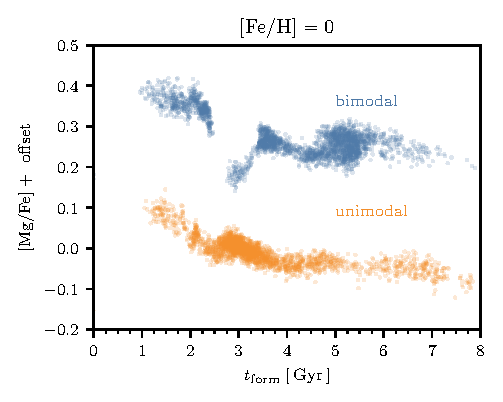
\includegraphics[width=\columnwidth]{alpha_vs_tform.pdf}
  \caption{\textbf{In the bimodal simulation, a gap in stellar ages is briefly followed by the formation of $\alpha$-deficient star particles.} The formation times and \MgFe{} values of star particles in the bimodal (blue) and unimodal (orange) simulations. In the unimodal simulation, no gap is present and there is briefly the formation of $\alpha$-enhanced star particles at the same time. The \MgFe{} values of the unimodal simulation have been offset by $-0.3$ for clarity.}
  \label{fig:alpha_vs_tform}
\end{figure}
